\section{Results}
\label{sec:results}

The results are separated by gas, but not by monitoring station. We present
more detailed results for only one (Tijuca station was chosen randomly), and after aggregated results
considering all the stations. This is done because we have more than
a hundred models to analyse. To deal with this diversity, the steps
(hyperparameters choice and evaluation) are automated. We are
making predictions one hour ahead and it is possible to compare with one day
ahead models. After this, we will have a best model for each gas and each
station (23 on total). 

\subsection{Tijuca monitoring station}

The results follow the order specified in the above summary for each pollutant. 

\subsubsection{O\texorpdfstring{$_3$}{3}}

{\em Simple linear regression}

\vspace{2mm}

Applying the simple linear regression, the $R^2$ in the testing set was 0.837,
what appears to be a good start fitting. The variable with greater t-statistic
was O$_3$ shifted by one hour. Other features with great t-statistic (more than
20) was, in
order, wind speedy, ozone lag 2, hour sin, UR, ozone lag 24, hour cos, and RS.
This is interesting because we have already observed the hourly seasonality
and by the formation of ozone, RS is expected to influence (not necessarily
linearly). The shifts were expected by the autocorrelation graph. Only some few features (3) had p-value greater that 0.05. The
F-statistic considering all variables was practically zero. One important
problem with this approach was the very big condition number (3.4e+06) given
the observed multicollinearity. Figure \ref{fig:histogram-residuals-slr} shows
the histogram of the residuals very similar to a normal distribution (as
assumed by the model).The kurtosis was nearly 3, while the skewness around
0.22. Jarque-Bera rejects the null hypotheses that skew and kurt are the same
as normal distribution, however.  The fitting result in testing data can be
partially observed in Figure \ref{fig:observed-fitting-ozone-tijuca}. Looking
at Figure  \ref{fig:observed-vs-residual-linear-regression}, as larger the
observed ozone gets, the more underestimated the prediction is.

\begin{figure}
    \centering
    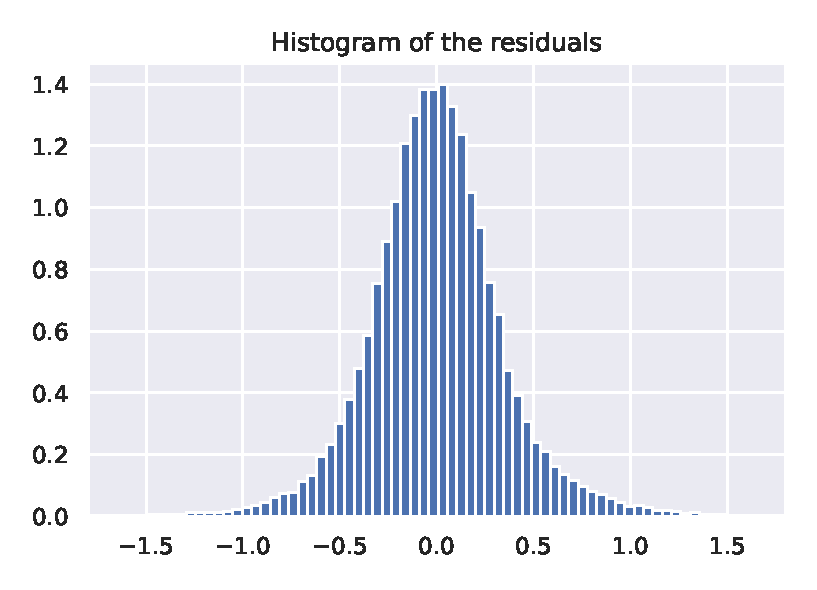
\includegraphics[width=0.45\textwidth]{histogram_residuals_slr.eps}
    \caption{Histogram of the residuals of simple linear regression model.}
    \label{fig:histogram-residuals-slr}
\end{figure}

\begin{figure}[!ht]
    \centering
    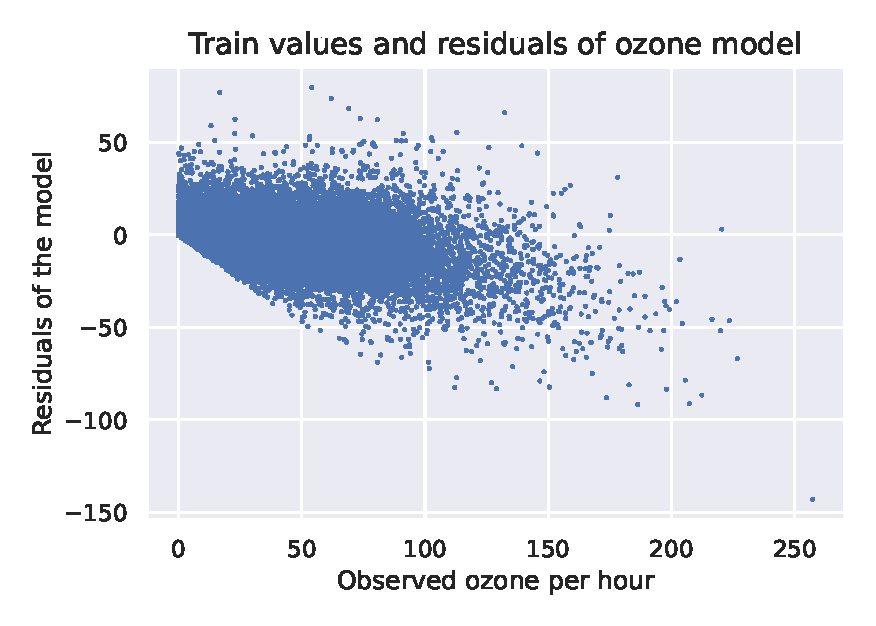
\includegraphics[width=0.45\textwidth]{observed-vs-residuals-linear-regression.eps}
    \caption{Simple linear regression residuals plotted against
    observed ozone values.}
    \label{fig:observed-vs-residual-linear-regression}
\end{figure}

When the lags 1 and 2 are removed, that is, only using the lag 24, the metrics
get much worse. In special, $R^2$ is around 0.49. Figure \ref{fig:r2-test-lag}
presents how the linear models performs badly when the first lags are removed.


\begin{figure}[!ht]
    \centering
    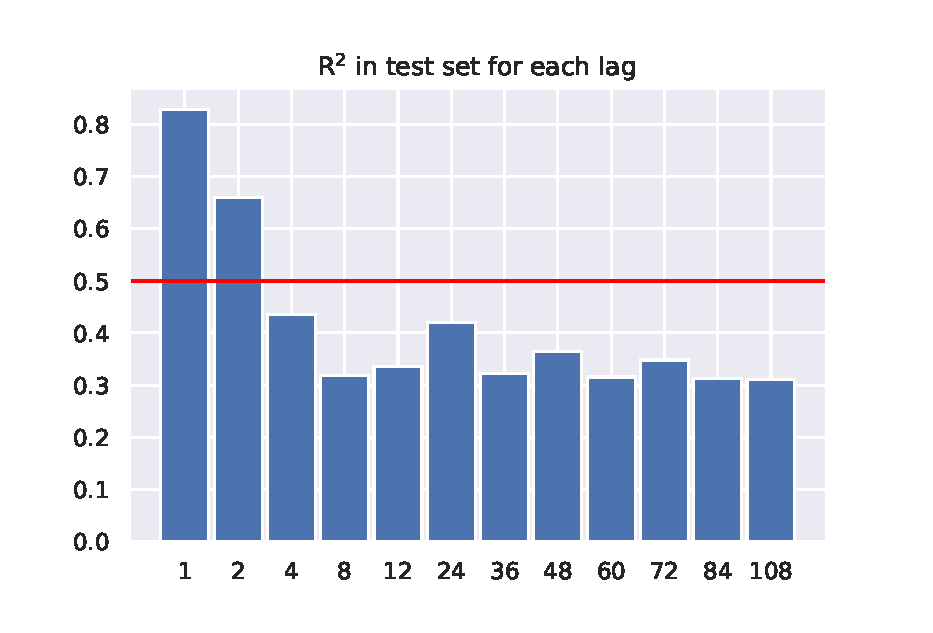
\includegraphics[width=0.45\textwidth]{r2_test_per_lag.eps}
    \caption{Removing all lag variables, adding only one per time, and calculating the R$^2$ in the test set.}
    \label{fig:r2-test-lag}
\end{figure}

\begin{figure*}[!ht]
    \centering
    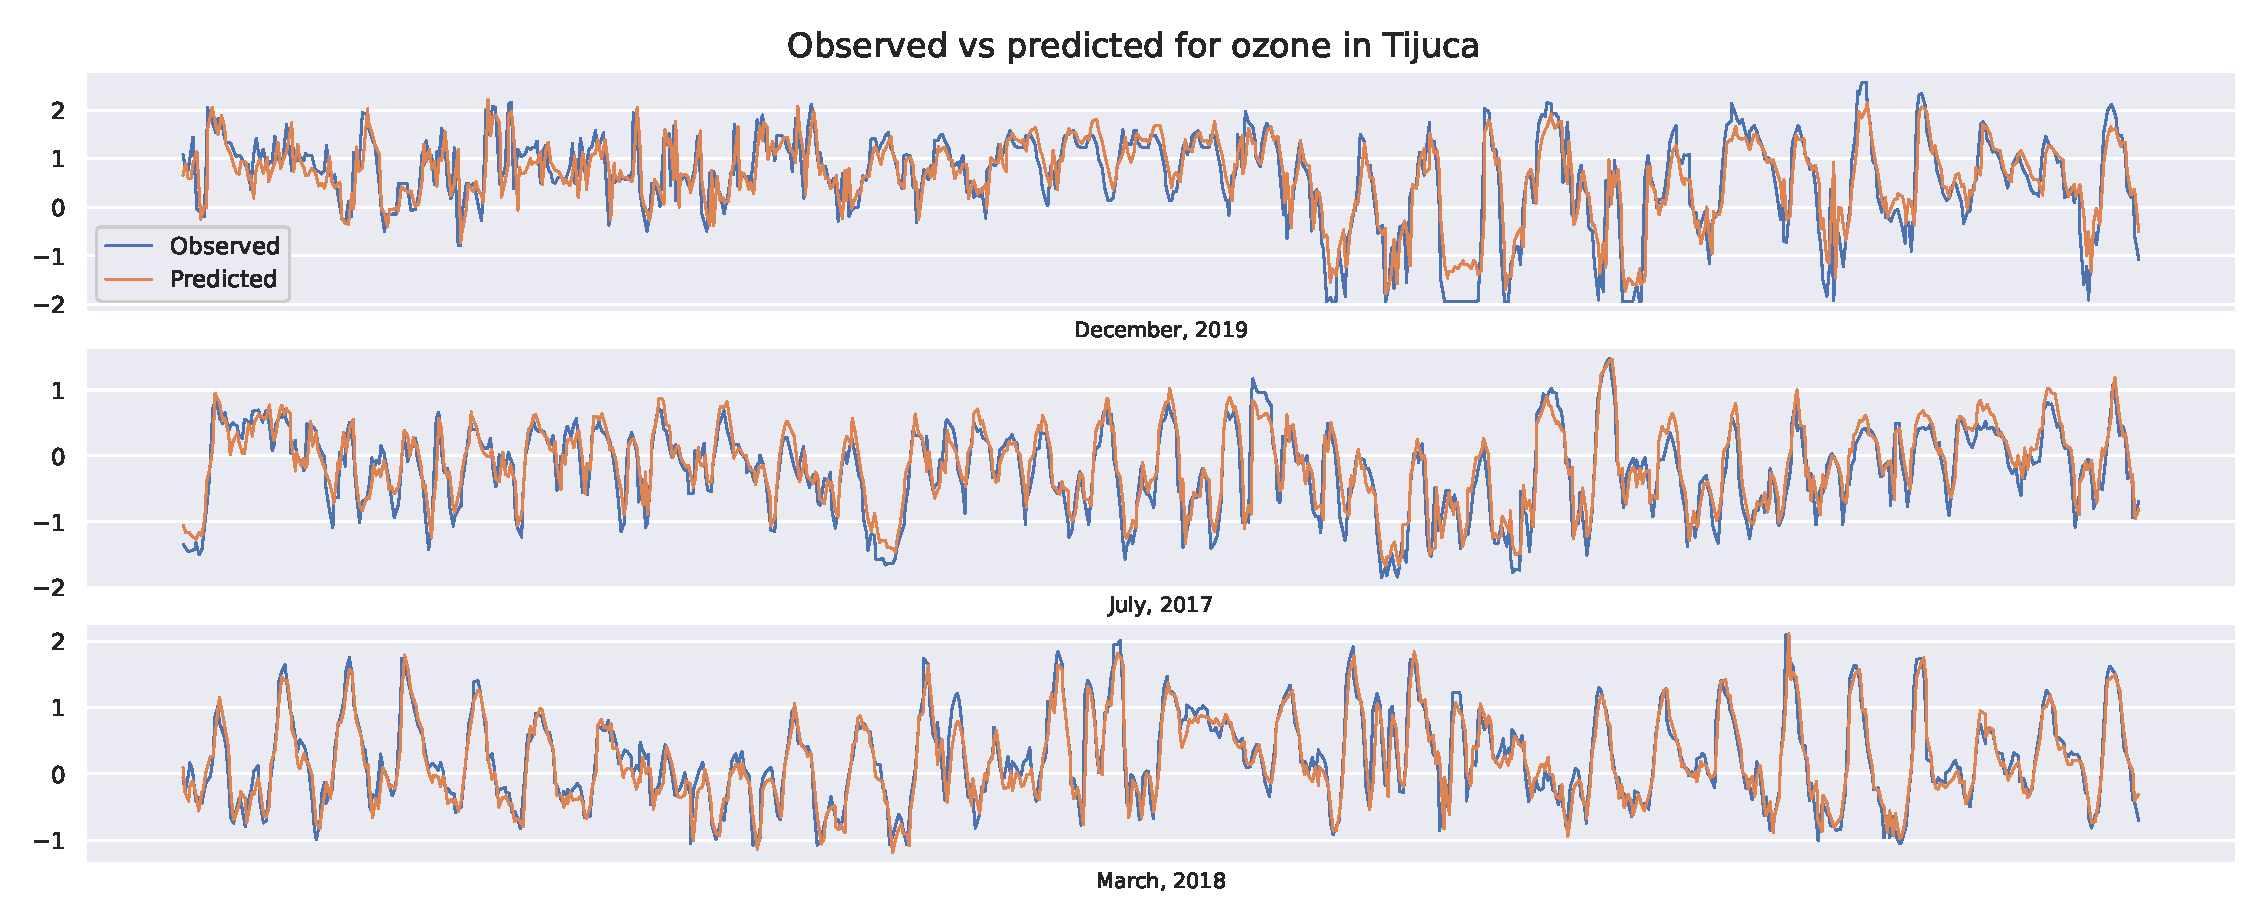
\includegraphics[width=\textwidth]{observed-fitting-ozone-tijuca.eps}
    \caption{Observed and predicted ozone values for different months in Tijuca.}
    \label{fig:observed-fitting-ozone-tijuca}
\end{figure*}

\vspace{2mm}

{\em Elastic-net regression}

\vspace{2mm}

One important observation is that the interaction terms make the metrics worse
in the pure linear regression and are disregarded for that reason. In this
case, they improve a lot. There are 376 features considering the polynomial
and interactions. The hyperparameters were set to $\alpha = 2$ and
$w_{l1} = 0.9$, what force several parameters to be zero. Only 6\% of the
variables ended to be non null. The result was interesting because all the non
zero coefficients were related to interactions with the {\tt year} variable.
This is related to Figure \ref{fig:time-series-gases-year}. $R^2$ in the test
set was 0.838, a few more than the simple linear regression. The histogram of
the residuals are similar to Figure \ref{fig:histogram-residuals-slr}, and
skewness and kurtosis too.

\begin{remark}
    Without interaction terms, the $R^2$ was around 0.5 and $\alpha$ was
    almost 0. 
\end{remark}

\vspace{2mm}

{\em Feature selection + Linear regression}

\vspace{2mm}

Feature selection was performed (proper code) with 5-Fold cross validation and
threshold equals to 0.001, that is, if the $R^2$ score improves less than
0.001, the features stop to be added in the best subset. The chosen features
were {\tt year * O3\_lag1}, {\tt RS}, {\tt RS * hour\_cos}, {\tt year *
Vel\_Vento}, {\tt O3\_lag2}, {\tt year O3\_MA24}, {\tt hour\_cos \* PM10\_lag1},
{\tt RS * Temp}, {\tt RS * O3\_lag2}, and {\tt O3\_lag1**2}. Note that it is
very different from those selected by elastic net. All the variables had
p-value less than 0.001, histogram similar to
\ref{fig:histogram-residuals-slr}, and Jarque-Bera indicating non-normality.
The $R^2$ in testing data was 0.848. 

Other important consideration is that the condition number is still big:
9.72e+03, despite being smaller than in simple regression case. After
calculating the Pearson correlation between the best variables, {\tt O3\_lag2}
and {\tt year * O3\_lag1} have more than 0.8, what was expected and even used.
Some experiments were conducted to reduce this value, but none was successful.
It appears that all variables are strongly (and linearly) related but also
add some information to prediction (at least a subset of them). This is bad
for the interpretation of the coefficients, since its identifiability cannot
be proved.  

\begin{remark}
    Solar radiation had a positive coefficient, so when it increases one unit
    of standard deviation, the ozone grows too. 
\end{remark}

\vspace{2mm}

{\em Support Vector Regression}

\vspace{2mm}

We remember that this model is computationally very costly, so its optimality
is not reached. From the cross validation, the best hyperparameters were
$\epsilon = 0.2$ and $C = 1.0$. With these values, we perform the linear SVR and
the SVR with kernel RBF only to compare them (it is practically
impossible to handle this amount of data with grid search when RBF kernel is
used in only one computer).

Setting those parameters, SVR with kernel RBF took 6min 28s (CPU time), while
Linear SVR 13.1s (CPU time). With RBF kernel, the $R^2$ in testing data was 0.78 and
with linear, it was 0.839. Looking at $R^2$ in training data, we observe that
the non-linear kernel suffered with over-fitting. Residues have not changed
much from the latest graphs, neither kurtosis nor skewness.

Considering the dataset with polynomial and interaction terms, we used the
best features chosen by Forward Feature Selection in the linear regression case. The
$R^2$ in testing data grew to 0.848 (the same as in the linear regression
case). The hyperparameters were not changed because a grid search did not
change. Feature selection could be done with this model too, but it would be
too costly. Finally, the SVR with RBF kernel was performed with the best
features. The $R^2$ in testing set was 0.851. 

\vspace{2mm}

{\em Random Forest} 

\vspace{2mm}

This algorithm is also very costly for large datasets, specially caused by the
choice of $s$ or other parameters, such as, max depth. This makes it harder to
do grid search to choose the best parameters. First, we consider that $s \in
\{10, 20, 50, 100\}$, $c \in \{0.0, 0.0001, 0.001, 0.01, 0.1, 1\}$, and $B =
100$. The chosen parameters were $s = 10$ and $c = 0$ (no regularization).
With this setting, $R^2$ in testing set was 0.848. From this result, we change
the the grid search to $s \in
\{2, 5, 8\}$ and $c \in \{0.0, 0.01, 1\}$. As expected, the selected were $c =
0.0$ and $s = 2$. However, despite needing more time, the $R^2$ in the testing
set did not improve. 


\subsubsection{CO}

\subsubsection{PM\texorpdfstring{$_{10}$}{10}}

\subsubsection{AIQ}

\subsection{Aggregated results}

\subsubsection{O\texorpdfstring{$_3$}{3}}

\subsubsection{PM\texorpdfstring{$_{10}$}{10}}

\subsubsection{CO}

\subsubsection{AIQ}

\subsection{Model for other locations}

Here, we want to make predictions about pollutant levels at other not measured
sites. Given that each location has a specific model, the prediction
is the weighted mean regarding each prediction 

\begin{enumerate}
    \item Testar estacionaridade de cada série;
\end{enumerate}



\section{Discussion and Future work}
\label{sec:discussion}


\section{Conclusion}
\label{sec:conclusion}
